\RequirePackage{silence} % :-\
%    \WarningFilter{scrreprt}{Usage of package `titlesec'}
%    \WarningFilter{scrreprt}{Activating an ugly workaround}
%    \WarningFilter{titlesec}{Non standard sectioning command detected}
\documentclass[ twoside,openright,titlepage,numbers=noenddot,%1headlines,
headinclude,footinclude,cleardoublepage=empty,abstract=on,
BCOR=5mm,paper=a4,fontsize=11pt
]{scrreprt}
\usepackage{xspace}
\usepackage{minted}
% ****************************************************************************************************
% classicthesis-config.tex
% formerly known as loadpackages.sty, classicthesis-ldpkg.sty, and classicthesis-preamble.sty
% Use it at the beginning of your ClassicThesis.tex, or as a LaTeX Preamble
% in your ClassicThesis.{tex,lyx} with % ****************************************************************************************************
% classicthesis-config.tex
% formerly known as loadpackages.sty, classicthesis-ldpkg.sty, and classicthesis-preamble.sty
% Use it at the beginning of your ClassicThesis.tex, or as a LaTeX Preamble
% in your ClassicThesis.{tex,lyx} with % ****************************************************************************************************
% classicthesis-config.tex
% formerly known as loadpackages.sty, classicthesis-ldpkg.sty, and classicthesis-preamble.sty
% Use it at the beginning of your ClassicThesis.tex, or as a LaTeX Preamble
% in your ClassicThesis.{tex,lyx} with \input{classicthesis-config}
% ****************************************************************************************************
% If you like the classicthesis, then I would appreciate a postcard.
% My address can be found in the file ClassicThesis.pdf. A collection
% of the postcards I received so far is available online at
% http://postcards.miede.de
% ****************************************************************************************************


% ****************************************************************************************************
% 0. Set the encoding of your files. UTF-8 is the only sensible encoding nowadays. If you can't read
% äöüßáéçèê∂åëæƒÏ€ then change the encoding setting in your editor, not the line below. If your editor
% does not support utf8 use another editor!
% ****************************************************************************************************
\PassOptionsToPackage{utf8}{inputenc}
  \usepackage{inputenc}

\PassOptionsToPackage{T1}{fontenc} % T2A for cyrillics
  \usepackage{fontenc}


% ****************************************************************************************************
% 1. Configure classicthesis for your needs here, e.g., remove "drafting" below
% in order to deactivate the time-stamp on the pages
% (see ClassicThesis.pdf for more information):
% ****************************************************************************************************
\PassOptionsToPackage{
%  drafting=false,    % print version information on the bottom of the pages
  tocaligned=false, % the left column of the toc will be aligned (no indentation)
  dottedtoc=false,  % page numbers in ToC flushed right
  eulerchapternumbers=true, % use AMS Euler for chapter font (otherwise Palatino)
  linedheaders=false,       % chaper headers will have line above and beneath
  floatperchapter=true,     % numbering per chapter for all floats (i.e., Figure 1.1)
  eulermath=true,  % use awesome Euler fonts for mathematical formulae (only with pdfLaTeX)
  beramono=true,    % toggle a nice monospaced font (w/ bold)
  palatino=true,    % deactivate standard font for loading another one, see the last section at the end of this file for suggestions
  style=classicthesis % classicthesis, arsclassica
}{classicthesis}


% ****************************************************************************************************
% 2. Personal data and user ad-hoc commands (insert your own data here)
% ****************************************************************************************************
\newcommand{\myTitle}{Complex fluids in the GPU era\xspace}
\newcommand{\mySubtitle}{Algorithms and simulations\xspace}
\newcommand{\myDegree}{\xspace}
\newcommand{\myName}{Ra\'ul P. Pel\'aez\xspace}
\newcommand{\myProf}{Rafael Delgago Buscalioni\xspace}
\newcommand{\myOtherProf}{\xspace}
\newcommand{\mySupervisor}{\xspace}
\newcommand{\myFaculty}{Facultad de Ciencias\xspace}
\newcommand{\myDepartment}{Departamento de F\'isica Te\'orica de la Materia Condensada\xspace}
\newcommand{\myUni}{Universidad Aut\'onoma de Madrid\xspace}
\newcommand{\myLocation}{\xspace}
\newcommand{\myTime}{2020\xspace}
\newcommand{\myVersion}{0.1}


% ****************************************************************************************************
% 3. Loading some handy packages
% ****************************************************************************************************
% ********************************************************************
% Packages with options that might require adjustments
% ********************************************************************
\PassOptionsToPackage{american}{babel} % change this to your language(s), main language last
% Spanish languages need extra options in order to work with this template
%\PassOptionsToPackage{spanish,es-lcroman}{babel}
\usepackage{babel}

\usepackage{csquotes}
\PassOptionsToPackage{%
  %backend=biber,bibencoding=utf8, %instead of bibtex
  backend=bibtex8,bibencoding=ascii,%
  language=auto,%
  style=numeric-comp,%
  %style=authoryear-comp, % Author 1999, 2010
  %bibstyle=authoryear,dashed=false, % dashed: substitute rep. author with ---
  sorting=nyt, % name, year, title
  maxbibnames=10, % default: 3, et al.
  %backref=true,%
  natbib=true % natbib compatibility mode (\citep and \citet still work)
}{biblatex}
    \usepackage{biblatex}

\PassOptionsToPackage{fleqn}{amsmath}       % math environments and more by the AMS
  \usepackage{amsmath}

% ********************************************************************
% General useful packages
% ********************************************************************
\usepackage{graphicx} %
%\usepackage{scrhack} % fix warnings when using KOMA with listings package
\usepackage{xspace} % to get the spacing after macros right
% ****************************************************************************************************
%\usepackage{pgfplots} % External TikZ/PGF support (thanks to Andreas Nautsch)
%\usetikzlibrary{external}
%\tikzexternalize[mode=list and make, prefix=ext-tikz/]
% ****************************************************************************************************


% ****************************************************************************************************
% 4. Setup floats: tables, (sub)figures, and captions
% ****************************************************************************************************
\usepackage{tabularx} % better tables
  \setlength{\extrarowheight}{3pt} % increase table row height
%\newcommand{\tableheadline}[1]{\multicolumn{1}{l}{\spacedlowsmallcaps{#1}}}
%\newcommand{\myfloatalign}{\centering} % to be used with each float for alignment
\usepackage{subfig}
% ****************************************************************************************************


% ****************************************************************************************************
% 5. Setup code listings
% ****************************************************************************************************
\usepackage{listings}
%\lstset{emph={trueIndex,root},emphstyle=\color{BlueViolet}}%\underbar} % for special keywords
%\lstset{language=[LaTeX]Tex,%C++,
%  morekeywords={PassOptionsToPackage,selectlanguage},
%  keywordstyle=\color{RoyalBlue},%\bfseries,
%  basicstyle=\small\ttfamily,
%  %identifierstyle=\color{NavyBlue},
%  commentstyle=\color{Green}\ttfamily,
%  stringstyle=\rmfamily,
%  numbers=none,%left,%
%  numberstyle=\scriptsize,%\tiny
%  stepnumber=5,
%  numbersep=8pt,
%  showstringspaces=false,
%  breaklines=true,
%  %frameround=ftff,
%  %frame=single,
%  belowcaptionskip=.75\baselineskip
%  %frame=L
%}
% ****************************************************************************************************




% ****************************************************************************************************
% 6. Last calls before the bar closes
% ****************************************************************************************************
% ********************************************************************
% Her Majesty herself
% ********************************************************************
\usepackage{classicthesis}


% ********************************************************************
% Fine-tune hyperreferences (hyperref should be called last)
% ********************************************************************
\hypersetup{%
%  %draft, % hyperref's draft mode, for printing see below
  colorlinks=true
  %, linktocpage=true, pdfstartpage=3, pdfstartview=FitV,%
%  % uncomment the following line if you want to have black links (e.g., for printing)
%  %colorlinks=false, linktocpage=false, pdfstartpage=3, pdfstartview=FitV, pdfborder={0 0 0},%
%  breaklinks=true, pageanchor=true,%
%  pdfpagemode=UseNone, %
%  % pdfpagemode=UseOutlines,%
%  plainpages=false, bookmarksnumbered, bookmarksopen=true, bookmarksopenlevel=1,%
%  hypertexnames=true, pdfhighlight=/O,%nesting=true,%frenchlinks,%
%  urlcolor=CTurl, linkcolor=CTlink, citecolor=CTcitation, %pagecolor=RoyalBlue,%
%  %urlcolor=Black, linkcolor=Black, citecolor=Black, %pagecolor=Black,%
%  pdftitle={\myTitle},%
%  pdfauthor={\textcopyright\ \myName, \myUni, \myFaculty},%
%  pdfsubject={},%
%  pdfkeywords={},%
%  pdfcreator={pdfLaTeX},%
%  pdfproducer={LaTeX with hyperref and classicthesis}%
}


% ********************************************************************
% Setup autoreferences (hyperref and babel)
% ********************************************************************
% There are some issues regarding autorefnames
% http://www.tex.ac.uk/cgi-bin/texfaq2html?label=latexwords
% you have to redefine the macros for the
% language you use, e.g., american, ngerman
% (as chosen when loading babel/AtBeginDocument)
% ********************************************************************
%\makeatletter
%\@ifpackageloaded{babel}%
%  {%
%    \addto\extrasamerican{%
%      \renewcommand*{\figureautorefname}{Figure}%
%      \renewcommand*{\tableautorefname}{Table}%
%      \renewcommand*{\partautorefname}{Part}%
%      \renewcommand*{\chapterautorefname}{Chapter}%
%      \renewcommand*{\sectionautorefname}{Section}%
%      \renewcommand*{\subsectionautorefname}{Section}%
%      \renewcommand*{\subsubsectionautorefname}{Section}%
%    }%
%     % Fix to getting autorefs for subfigures right (thanks to Belinda Vogt for changing the definition)
%      \providecommand{\subfigureautorefname}{\figureautorefname}%
%    }{\relax}
%\makeatother


% ********************************************************************
% Development Stuff
% ********************************************************************
%\listfiles
%\PassOptionsToPackage{l2tabu,orthodox,abort}{nag}
%  \usepackage{nag}
%\PassOptionsToPackage{warning, all}{onlyamsmath}
%  \usepackage{onlyamsmath}


% ****************************************************************************************************
% 7. Further adjustments (experimental)
% ****************************************************************************************************
% ********************************************************************
% Changing the text area
% ********************************************************************
%\areaset[current]{312pt}{761pt} % 686 (factor 2.2) + 33 head + 42 head \the\footskip
%\setlength{\marginparwidth}{7em}%
%\setlength{\marginparsep}{2em}%

% ********************************************************************
% Using different fonts
% ********************************************************************
%\usepackage[oldstylenums]{kpfonts} % oldstyle notextcomp
% \usepackage[osf]{libertine}
%\usepackage[light,condensed,math]{iwona}
%\renewcommand{\sfdefault}{iwona}
%\usepackage{lmodern} % <-- no osf support :-(
%\usepackage{cfr-lm} %
%\usepackage[urw-garamond]{mathdesign} <-- no osf support :-(
%\usepackage[default,osfigures]{opensans} % scale=0.95
%\usepackage[sfdefault]{FiraSans}
% \usepackage[opticals,mathlf]{MinionPro} % onlytext
% ********************************************************************
%\usepackage[largesc,osf]{newpxtext}
%\linespread{1.05} % a bit more for Palatino
% Used to fix these:
% https://bitbucket.org/amiede/classicthesis/issues/139/italics-in-pallatino-capitals-chapter
% https://bitbucket.org/amiede/classicthesis/issues/45/problema-testatine-su-classicthesis-style
% ********************************************************************
% ****************************************************************************************************

% ****************************************************************************************************
% If you like the classicthesis, then I would appreciate a postcard.
% My address can be found in the file ClassicThesis.pdf. A collection
% of the postcards I received so far is available online at
% http://postcards.miede.de
% ****************************************************************************************************


% ****************************************************************************************************
% 0. Set the encoding of your files. UTF-8 is the only sensible encoding nowadays. If you can't read
% äöüßáéçèê∂åëæƒÏ€ then change the encoding setting in your editor, not the line below. If your editor
% does not support utf8 use another editor!
% ****************************************************************************************************
\PassOptionsToPackage{utf8}{inputenc}
  \usepackage{inputenc}

\PassOptionsToPackage{T1}{fontenc} % T2A for cyrillics
  \usepackage{fontenc}


% ****************************************************************************************************
% 1. Configure classicthesis for your needs here, e.g., remove "drafting" below
% in order to deactivate the time-stamp on the pages
% (see ClassicThesis.pdf for more information):
% ****************************************************************************************************
\PassOptionsToPackage{
%  drafting=false,    % print version information on the bottom of the pages
  tocaligned=false, % the left column of the toc will be aligned (no indentation)
  dottedtoc=false,  % page numbers in ToC flushed right
  eulerchapternumbers=true, % use AMS Euler for chapter font (otherwise Palatino)
  linedheaders=false,       % chaper headers will have line above and beneath
  floatperchapter=true,     % numbering per chapter for all floats (i.e., Figure 1.1)
  eulermath=true,  % use awesome Euler fonts for mathematical formulae (only with pdfLaTeX)
  beramono=true,    % toggle a nice monospaced font (w/ bold)
  palatino=true,    % deactivate standard font for loading another one, see the last section at the end of this file for suggestions
  style=classicthesis % classicthesis, arsclassica
}{classicthesis}


% ****************************************************************************************************
% 2. Personal data and user ad-hoc commands (insert your own data here)
% ****************************************************************************************************
\newcommand{\myTitle}{Complex fluids in the GPU era\xspace}
\newcommand{\mySubtitle}{Algorithms and simulations\xspace}
\newcommand{\myDegree}{\xspace}
\newcommand{\myName}{Ra\'ul P. Pel\'aez\xspace}
\newcommand{\myProf}{Rafael Delgago Buscalioni\xspace}
\newcommand{\myOtherProf}{\xspace}
\newcommand{\mySupervisor}{\xspace}
\newcommand{\myFaculty}{Facultad de Ciencias\xspace}
\newcommand{\myDepartment}{Departamento de F\'isica Te\'orica de la Materia Condensada\xspace}
\newcommand{\myUni}{Universidad Aut\'onoma de Madrid\xspace}
\newcommand{\myLocation}{\xspace}
\newcommand{\myTime}{2020\xspace}
\newcommand{\myVersion}{0.1}


% ****************************************************************************************************
% 3. Loading some handy packages
% ****************************************************************************************************
% ********************************************************************
% Packages with options that might require adjustments
% ********************************************************************
\PassOptionsToPackage{american}{babel} % change this to your language(s), main language last
% Spanish languages need extra options in order to work with this template
%\PassOptionsToPackage{spanish,es-lcroman}{babel}
\usepackage{babel}

\usepackage{csquotes}
\PassOptionsToPackage{%
  %backend=biber,bibencoding=utf8, %instead of bibtex
  backend=bibtex8,bibencoding=ascii,%
  language=auto,%
  style=numeric-comp,%
  %style=authoryear-comp, % Author 1999, 2010
  %bibstyle=authoryear,dashed=false, % dashed: substitute rep. author with ---
  sorting=nyt, % name, year, title
  maxbibnames=10, % default: 3, et al.
  %backref=true,%
  natbib=true % natbib compatibility mode (\citep and \citet still work)
}{biblatex}
    \usepackage{biblatex}

\PassOptionsToPackage{fleqn}{amsmath}       % math environments and more by the AMS
  \usepackage{amsmath}

% ********************************************************************
% General useful packages
% ********************************************************************
\usepackage{graphicx} %
%\usepackage{scrhack} % fix warnings when using KOMA with listings package
\usepackage{xspace} % to get the spacing after macros right
% ****************************************************************************************************
%\usepackage{pgfplots} % External TikZ/PGF support (thanks to Andreas Nautsch)
%\usetikzlibrary{external}
%\tikzexternalize[mode=list and make, prefix=ext-tikz/]
% ****************************************************************************************************


% ****************************************************************************************************
% 4. Setup floats: tables, (sub)figures, and captions
% ****************************************************************************************************
\usepackage{tabularx} % better tables
  \setlength{\extrarowheight}{3pt} % increase table row height
%\newcommand{\tableheadline}[1]{\multicolumn{1}{l}{\spacedlowsmallcaps{#1}}}
%\newcommand{\myfloatalign}{\centering} % to be used with each float for alignment
\usepackage{subfig}
% ****************************************************************************************************


% ****************************************************************************************************
% 5. Setup code listings
% ****************************************************************************************************
\usepackage{listings}
%\lstset{emph={trueIndex,root},emphstyle=\color{BlueViolet}}%\underbar} % for special keywords
%\lstset{language=[LaTeX]Tex,%C++,
%  morekeywords={PassOptionsToPackage,selectlanguage},
%  keywordstyle=\color{RoyalBlue},%\bfseries,
%  basicstyle=\small\ttfamily,
%  %identifierstyle=\color{NavyBlue},
%  commentstyle=\color{Green}\ttfamily,
%  stringstyle=\rmfamily,
%  numbers=none,%left,%
%  numberstyle=\scriptsize,%\tiny
%  stepnumber=5,
%  numbersep=8pt,
%  showstringspaces=false,
%  breaklines=true,
%  %frameround=ftff,
%  %frame=single,
%  belowcaptionskip=.75\baselineskip
%  %frame=L
%}
% ****************************************************************************************************




% ****************************************************************************************************
% 6. Last calls before the bar closes
% ****************************************************************************************************
% ********************************************************************
% Her Majesty herself
% ********************************************************************
\usepackage{classicthesis}


% ********************************************************************
% Fine-tune hyperreferences (hyperref should be called last)
% ********************************************************************
\hypersetup{%
%  %draft, % hyperref's draft mode, for printing see below
  colorlinks=true
  %, linktocpage=true, pdfstartpage=3, pdfstartview=FitV,%
%  % uncomment the following line if you want to have black links (e.g., for printing)
%  %colorlinks=false, linktocpage=false, pdfstartpage=3, pdfstartview=FitV, pdfborder={0 0 0},%
%  breaklinks=true, pageanchor=true,%
%  pdfpagemode=UseNone, %
%  % pdfpagemode=UseOutlines,%
%  plainpages=false, bookmarksnumbered, bookmarksopen=true, bookmarksopenlevel=1,%
%  hypertexnames=true, pdfhighlight=/O,%nesting=true,%frenchlinks,%
%  urlcolor=CTurl, linkcolor=CTlink, citecolor=CTcitation, %pagecolor=RoyalBlue,%
%  %urlcolor=Black, linkcolor=Black, citecolor=Black, %pagecolor=Black,%
%  pdftitle={\myTitle},%
%  pdfauthor={\textcopyright\ \myName, \myUni, \myFaculty},%
%  pdfsubject={},%
%  pdfkeywords={},%
%  pdfcreator={pdfLaTeX},%
%  pdfproducer={LaTeX with hyperref and classicthesis}%
}


% ********************************************************************
% Setup autoreferences (hyperref and babel)
% ********************************************************************
% There are some issues regarding autorefnames
% http://www.tex.ac.uk/cgi-bin/texfaq2html?label=latexwords
% you have to redefine the macros for the
% language you use, e.g., american, ngerman
% (as chosen when loading babel/AtBeginDocument)
% ********************************************************************
%\makeatletter
%\@ifpackageloaded{babel}%
%  {%
%    \addto\extrasamerican{%
%      \renewcommand*{\figureautorefname}{Figure}%
%      \renewcommand*{\tableautorefname}{Table}%
%      \renewcommand*{\partautorefname}{Part}%
%      \renewcommand*{\chapterautorefname}{Chapter}%
%      \renewcommand*{\sectionautorefname}{Section}%
%      \renewcommand*{\subsectionautorefname}{Section}%
%      \renewcommand*{\subsubsectionautorefname}{Section}%
%    }%
%     % Fix to getting autorefs for subfigures right (thanks to Belinda Vogt for changing the definition)
%      \providecommand{\subfigureautorefname}{\figureautorefname}%
%    }{\relax}
%\makeatother


% ********************************************************************
% Development Stuff
% ********************************************************************
%\listfiles
%\PassOptionsToPackage{l2tabu,orthodox,abort}{nag}
%  \usepackage{nag}
%\PassOptionsToPackage{warning, all}{onlyamsmath}
%  \usepackage{onlyamsmath}


% ****************************************************************************************************
% 7. Further adjustments (experimental)
% ****************************************************************************************************
% ********************************************************************
% Changing the text area
% ********************************************************************
%\areaset[current]{312pt}{761pt} % 686 (factor 2.2) + 33 head + 42 head \the\footskip
%\setlength{\marginparwidth}{7em}%
%\setlength{\marginparsep}{2em}%

% ********************************************************************
% Using different fonts
% ********************************************************************
%\usepackage[oldstylenums]{kpfonts} % oldstyle notextcomp
% \usepackage[osf]{libertine}
%\usepackage[light,condensed,math]{iwona}
%\renewcommand{\sfdefault}{iwona}
%\usepackage{lmodern} % <-- no osf support :-(
%\usepackage{cfr-lm} %
%\usepackage[urw-garamond]{mathdesign} <-- no osf support :-(
%\usepackage[default,osfigures]{opensans} % scale=0.95
%\usepackage[sfdefault]{FiraSans}
% \usepackage[opticals,mathlf]{MinionPro} % onlytext
% ********************************************************************
%\usepackage[largesc,osf]{newpxtext}
%\linespread{1.05} % a bit more for Palatino
% Used to fix these:
% https://bitbucket.org/amiede/classicthesis/issues/139/italics-in-pallatino-capitals-chapter
% https://bitbucket.org/amiede/classicthesis/issues/45/problema-testatine-su-classicthesis-style
% ********************************************************************
% ****************************************************************************************************

% ****************************************************************************************************
% If you like the classicthesis, then I would appreciate a postcard.
% My address can be found in the file ClassicThesis.pdf. A collection
% of the postcards I received so far is available online at
% http://postcards.miede.de
% ****************************************************************************************************


% ****************************************************************************************************
% 0. Set the encoding of your files. UTF-8 is the only sensible encoding nowadays. If you can't read
% äöüßáéçèê∂åëæƒÏ€ then change the encoding setting in your editor, not the line below. If your editor
% does not support utf8 use another editor!
% ****************************************************************************************************
\PassOptionsToPackage{utf8}{inputenc}
  \usepackage{inputenc}

\PassOptionsToPackage{T1}{fontenc} % T2A for cyrillics
  \usepackage{fontenc}


% ****************************************************************************************************
% 1. Configure classicthesis for your needs here, e.g., remove "drafting" below
% in order to deactivate the time-stamp on the pages
% (see ClassicThesis.pdf for more information):
% ****************************************************************************************************
\PassOptionsToPackage{
%  drafting=false,    % print version information on the bottom of the pages
  tocaligned=false, % the left column of the toc will be aligned (no indentation)
  dottedtoc=false,  % page numbers in ToC flushed right
  eulerchapternumbers=true, % use AMS Euler for chapter font (otherwise Palatino)
  linedheaders=false,       % chaper headers will have line above and beneath
  floatperchapter=true,     % numbering per chapter for all floats (i.e., Figure 1.1)
  eulermath=true,  % use awesome Euler fonts for mathematical formulae (only with pdfLaTeX)
  beramono=true,    % toggle a nice monospaced font (w/ bold)
  palatino=true,    % deactivate standard font for loading another one, see the last section at the end of this file for suggestions
  style=classicthesis % classicthesis, arsclassica
}{classicthesis}


% ****************************************************************************************************
% 2. Personal data and user ad-hoc commands (insert your own data here)
% ****************************************************************************************************
\newcommand{\myTitle}{Complex fluids in the GPU era\xspace}
\newcommand{\mySubtitle}{Algorithms and simulations\xspace}
\newcommand{\myDegree}{\xspace}
\newcommand{\myName}{Ra\'ul P. Pel\'aez\xspace}
\newcommand{\myProf}{Rafael Delgago Buscalioni\xspace}
\newcommand{\myOtherProf}{\xspace}
\newcommand{\mySupervisor}{\xspace}
\newcommand{\myFaculty}{Facultad de Ciencias\xspace}
\newcommand{\myDepartment}{Departamento de F\'isica Te\'orica de la Materia Condensada\xspace}
\newcommand{\myUni}{Universidad Aut\'onoma de Madrid\xspace}
\newcommand{\myLocation}{\xspace}
\newcommand{\myTime}{2020\xspace}
\newcommand{\myVersion}{0.1}


% ****************************************************************************************************
% 3. Loading some handy packages
% ****************************************************************************************************
% ********************************************************************
% Packages with options that might require adjustments
% ********************************************************************
\PassOptionsToPackage{american}{babel} % change this to your language(s), main language last
% Spanish languages need extra options in order to work with this template
%\PassOptionsToPackage{spanish,es-lcroman}{babel}
\usepackage{babel}

\usepackage{csquotes}
\PassOptionsToPackage{%
  %backend=biber,bibencoding=utf8, %instead of bibtex
  backend=bibtex8,bibencoding=ascii,%
  language=auto,%
  style=numeric-comp,%
  %style=authoryear-comp, % Author 1999, 2010
  %bibstyle=authoryear,dashed=false, % dashed: substitute rep. author with ---
  sorting=nyt, % name, year, title
  maxbibnames=10, % default: 3, et al.
  %backref=true,%
  natbib=true % natbib compatibility mode (\citep and \citet still work)
}{biblatex}
    \usepackage{biblatex}

\PassOptionsToPackage{fleqn}{amsmath}       % math environments and more by the AMS
  \usepackage{amsmath}

% ********************************************************************
% General useful packages
% ********************************************************************
\usepackage{graphicx} %
%\usepackage{scrhack} % fix warnings when using KOMA with listings package
\usepackage{xspace} % to get the spacing after macros right
% ****************************************************************************************************
%\usepackage{pgfplots} % External TikZ/PGF support (thanks to Andreas Nautsch)
%\usetikzlibrary{external}
%\tikzexternalize[mode=list and make, prefix=ext-tikz/]
% ****************************************************************************************************


% ****************************************************************************************************
% 4. Setup floats: tables, (sub)figures, and captions
% ****************************************************************************************************
\usepackage{tabularx} % better tables
  \setlength{\extrarowheight}{3pt} % increase table row height
%\newcommand{\tableheadline}[1]{\multicolumn{1}{l}{\spacedlowsmallcaps{#1}}}
%\newcommand{\myfloatalign}{\centering} % to be used with each float for alignment
\usepackage{subfig}
% ****************************************************************************************************


% ****************************************************************************************************
% 5. Setup code listings
% ****************************************************************************************************
\usepackage{listings}
%\lstset{emph={trueIndex,root},emphstyle=\color{BlueViolet}}%\underbar} % for special keywords
%\lstset{language=[LaTeX]Tex,%C++,
%  morekeywords={PassOptionsToPackage,selectlanguage},
%  keywordstyle=\color{RoyalBlue},%\bfseries,
%  basicstyle=\small\ttfamily,
%  %identifierstyle=\color{NavyBlue},
%  commentstyle=\color{Green}\ttfamily,
%  stringstyle=\rmfamily,
%  numbers=none,%left,%
%  numberstyle=\scriptsize,%\tiny
%  stepnumber=5,
%  numbersep=8pt,
%  showstringspaces=false,
%  breaklines=true,
%  %frameround=ftff,
%  %frame=single,
%  belowcaptionskip=.75\baselineskip
%  %frame=L
%}
% ****************************************************************************************************




% ****************************************************************************************************
% 6. Last calls before the bar closes
% ****************************************************************************************************
% ********************************************************************
% Her Majesty herself
% ********************************************************************
\usepackage{classicthesis}


% ********************************************************************
% Fine-tune hyperreferences (hyperref should be called last)
% ********************************************************************
\hypersetup{%
%  %draft, % hyperref's draft mode, for printing see below
  colorlinks=true
  %, linktocpage=true, pdfstartpage=3, pdfstartview=FitV,%
%  % uncomment the following line if you want to have black links (e.g., for printing)
%  %colorlinks=false, linktocpage=false, pdfstartpage=3, pdfstartview=FitV, pdfborder={0 0 0},%
%  breaklinks=true, pageanchor=true,%
%  pdfpagemode=UseNone, %
%  % pdfpagemode=UseOutlines,%
%  plainpages=false, bookmarksnumbered, bookmarksopen=true, bookmarksopenlevel=1,%
%  hypertexnames=true, pdfhighlight=/O,%nesting=true,%frenchlinks,%
%  urlcolor=CTurl, linkcolor=CTlink, citecolor=CTcitation, %pagecolor=RoyalBlue,%
%  %urlcolor=Black, linkcolor=Black, citecolor=Black, %pagecolor=Black,%
%  pdftitle={\myTitle},%
%  pdfauthor={\textcopyright\ \myName, \myUni, \myFaculty},%
%  pdfsubject={},%
%  pdfkeywords={},%
%  pdfcreator={pdfLaTeX},%
%  pdfproducer={LaTeX with hyperref and classicthesis}%
}


% ********************************************************************
% Setup autoreferences (hyperref and babel)
% ********************************************************************
% There are some issues regarding autorefnames
% http://www.tex.ac.uk/cgi-bin/texfaq2html?label=latexwords
% you have to redefine the macros for the
% language you use, e.g., american, ngerman
% (as chosen when loading babel/AtBeginDocument)
% ********************************************************************
%\makeatletter
%\@ifpackageloaded{babel}%
%  {%
%    \addto\extrasamerican{%
%      \renewcommand*{\figureautorefname}{Figure}%
%      \renewcommand*{\tableautorefname}{Table}%
%      \renewcommand*{\partautorefname}{Part}%
%      \renewcommand*{\chapterautorefname}{Chapter}%
%      \renewcommand*{\sectionautorefname}{Section}%
%      \renewcommand*{\subsectionautorefname}{Section}%
%      \renewcommand*{\subsubsectionautorefname}{Section}%
%    }%
%     % Fix to getting autorefs for subfigures right (thanks to Belinda Vogt for changing the definition)
%      \providecommand{\subfigureautorefname}{\figureautorefname}%
%    }{\relax}
%\makeatother


% ********************************************************************
% Development Stuff
% ********************************************************************
%\listfiles
%\PassOptionsToPackage{l2tabu,orthodox,abort}{nag}
%  \usepackage{nag}
%\PassOptionsToPackage{warning, all}{onlyamsmath}
%  \usepackage{onlyamsmath}


% ****************************************************************************************************
% 7. Further adjustments (experimental)
% ****************************************************************************************************
% ********************************************************************
% Changing the text area
% ********************************************************************
%\areaset[current]{312pt}{761pt} % 686 (factor 2.2) + 33 head + 42 head \the\footskip
%\setlength{\marginparwidth}{7em}%
%\setlength{\marginparsep}{2em}%

% ********************************************************************
% Using different fonts
% ********************************************************************
%\usepackage[oldstylenums]{kpfonts} % oldstyle notextcomp
% \usepackage[osf]{libertine}
%\usepackage[light,condensed,math]{iwona}
%\renewcommand{\sfdefault}{iwona}
%\usepackage{lmodern} % <-- no osf support :-(
%\usepackage{cfr-lm} %
%\usepackage[urw-garamond]{mathdesign} <-- no osf support :-(
%\usepackage[default,osfigures]{opensans} % scale=0.95
%\usepackage[sfdefault]{FiraSans}
% \usepackage[opticals,mathlf]{MinionPro} % onlytext
% ********************************************************************
%\usepackage[largesc,osf]{newpxtext}
%\linespread{1.05} % a bit more for Palatino
% Used to fix these:
% https://bitbucket.org/amiede/classicthesis/issues/139/italics-in-pallatino-capitals-chapter
% https://bitbucket.org/amiede/classicthesis/issues/45/problema-testatine-su-classicthesis-style
% ********************************************************************
% ****************************************************************************************************

\usepackage{amsmath}
\usepackage{bm}
\usepackage{hyperref}
\usepackage[acronym]{glossaries}
\usepackage[utf8]{inputenc}
\makeglossaries
\newacronym{UAMMD}{UAMMD}{Universaly Adaptable Multiscale Molecular Dynamics}
\newacronym{MD}{MD}{Molecular Dynamics}
\newacronym{BD}{BD}{Brownian Dynamics}
\newacronym{BDHI}{BDHI}{Brownian Dynamics with Hydrodynamic Interactions}
\newacronym{IBM}{IBM}{Immersed Boundary}
\newacronym{PSE}{PSE}{Positively Split Ewald}
\newacronym{FCM}{FCM}{Force Coupling Method}
\newacronym{ICM}{ICM}{Inertial Coupling Method}
\newacronym{FIB}{FIB}{Fluctuating Immersed Boundary}
\newacronym{DPD}{DPD}{Dissipative Particle Dynamics}
\newacronym{SPH}{SPH}{Smoothed Particle Hydrodynamics}
\newacronym{SE}{SE}{Spectral Ewald}
\newacronym{FFT}{FFT}{Fast Fourier Transform}
\newacronym{iFFT}{iFFT}{Inverse Fast Fourier Transform}
\newacronym{GPU}{GPU}{Graphical Processor Units}
\newacronym{GPGPU}{GPGPU}{General Purpose Computing on GPU}
\newacronym{RHS}{RHS}{Right Hand Side}
\newacronym{API}{API}{Application Programming Interface}


\renewcommand{\vec}[1]{\bm{#1}}
\newcommand{\uammd}{\gls{UAMMD}\xspace}
\newcommand{\gpu}{\gls{GPU}\xspace}

\DeclareMathOperator{\erf}{erf}

\addbibresource{Bibliography.bib}

%\hyphenation{put special hyphenation here}

\begin{document}
\frenchspacing
\raggedbottom
\selectlanguage{american} % american ngerman
%\renewcommand*{\bibname}{new name}
%\setbibpreamble{}
\pagenumbering{roman}
\pagestyle{plain}

%*******************************************************
% Little Dirty Titlepage
%*******************************************************
\thispagestyle{empty}
%\pdfbookmark[1]{Titel}{title}
%*******************************************************
\begin{center}
    \spacedlowsmallcaps{\myName} \\ \medskip

    \begingroup
        \color{CTtitle}\spacedallcaps{\myTitle}
    \endgroup
\end{center}



%*******************************************************
% Titlepage
%*******************************************************
\begin{titlepage}
    %\pdfbookmark[1]{\myTitle}{titlepage}
    % if you want the titlepage to be centered, uncomment and fine-tune the line below (KOMA classes environment)
    \begin{addmargin}[-1cm]{-3cm}
    \begin{center}
        \large

        \hfill

        \vfill

        \begingroup
            \color{CTtitle}\spacedallcaps{\myTitle} \\ \bigskip
        \endgroup

        \spacedlowsmallcaps{\myName}

        \vfill

        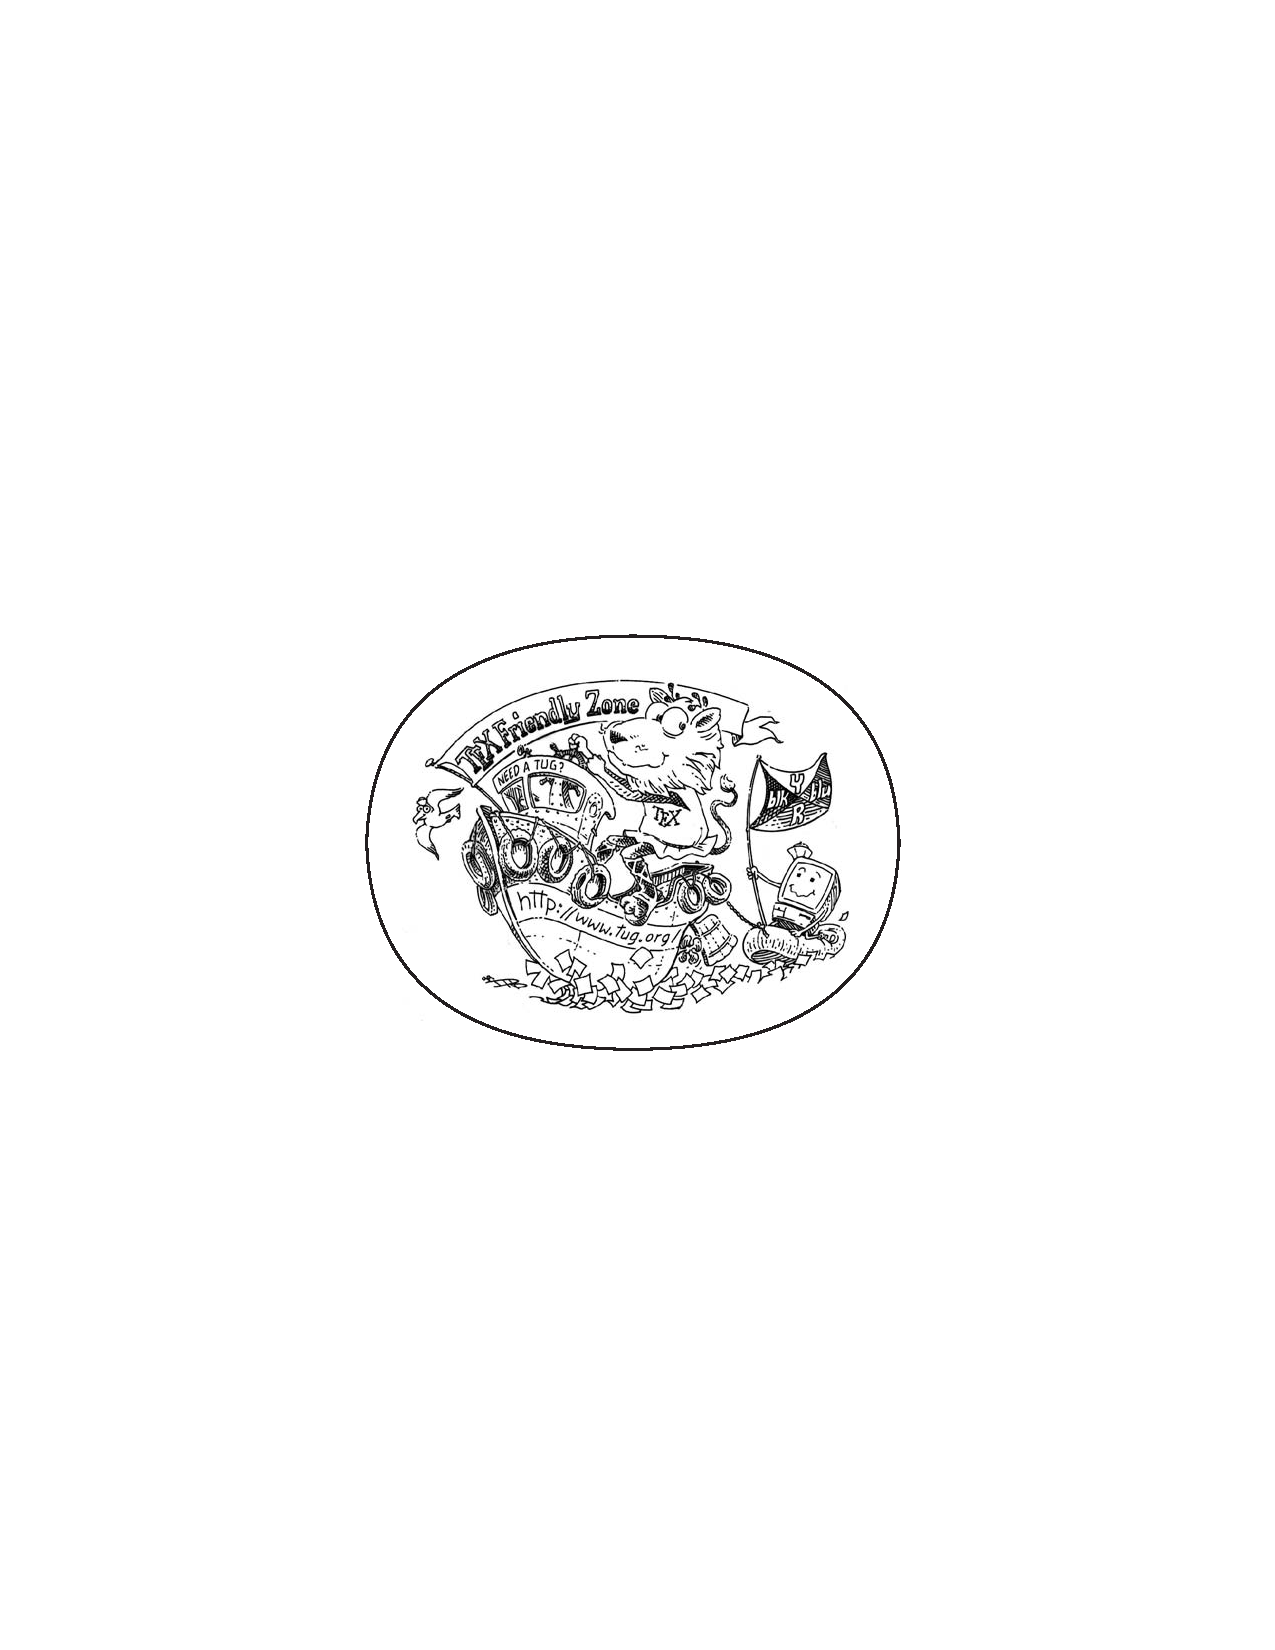
\includegraphics[width=6cm]{gfx/TFZsuperellipse_bw} \\ \medskip

        \mySubtitle \\ \medskip
        %\myDegree \\
        \myDepartment \\
        \myFaculty \\
        \myUni \\ \bigskip

        \myTime\ -- \myVersion

        \vfill

    \end{center}
  \end{addmargin}
\end{titlepage}

\thispagestyle{empty}

\hfill

\vfill

\noindent\myName: \textit{\myTitle,} \mySubtitle, %\myDegree,
\textcopyright\ \myTime

%\bigskip
%
%\noindent\spacedlowsmallcaps{Supervisors}: \\
%\myProf \\
%\myOtherProf \\
%\mySupervisor
%
%\medskip
%
%\noindent\spacedlowsmallcaps{Location}: \\
%\myLocation
%
%\medskip
%
%\noindent\spacedlowsmallcaps{Time Frame}: \\
%\myTime

\cleardoublepage%*******************************************************
% Dedication
%*******************************************************
\thispagestyle{empty}
\phantomsection
\pdfbookmark[1]{Dedication}{Dedication}

\vspace*{3cm}

\begin{center}
      This thing is complex... so complex not even God gets it.\\ \medskip
    --- Rafa Buscalioni
    \\ \medskip\medskip
        There is no way you are getting a quote for your stupid thesis\\ \medskip
    --- NVIDIA

\end{center}

\medskip

%\cleardoublepage\input{FrontBackmatter/Foreword}
\cleardoublepage%*******************************************************
% Abstract
%*******************************************************
%\renewcommand{\abstractname}{Abstract}
\pdfbookmark[1]{Abstract}{Abstract}
% \addcontentsline{toc}{chapter}{\tocEntry{Abstract}}
\begingroup
\let\clearpage\relax
\let\cleardoublepage\relax
\let\cleardoublepage\relax

\chapter*{Abstract}

Some abstract


\cleardoublepage%*******************************************************
% Publications
%*******************************************************
\pdfbookmark[1]{Publications}{publications}
\chapter*{Publications}
The following publications resulted from the development of this work
%\noindent Put your publications from the thesis here. The packages \texttt{multibib} or \texttt{bibtopic} etc. can be used to handle multiple different bibliographies in your document.

\begin{refsection}[ownpubs]
    \small
    \nocite{*} % is local to to the enclosing refsection
    \printbibliography[heading=none]
\end{refsection}

\cleardoublepage%*******************************************************
% Acknowledgments
%*******************************************************
\pdfbookmark[1]{Acknowledgments}{acknowledgments}

\begin{flushright}{\slshape}
\end{flushright}



\bigskip

\begingroup
\let\clearpage\relax
\let\cleardoublepage\relax
\let\cleardoublepage\relax
\chapter*{Acknowledgments}

\cleardoublepage%*******************************************************
% Table of Contents
%*******************************************************
\pagestyle{scrheadings}
%\phantomsection
\pdfbookmark[1]{\contentsname}{tableofcontents}
\setcounter{tocdepth}{2} % <-- 2 includes up to subsections in the ToC
\setcounter{secnumdepth}{3} % <-- 3 numbers up to subsubsections
\manualmark
\markboth{\spacedlowsmallcaps{\contentsname}}{\spacedlowsmallcaps{\contentsname}}
\tableofcontents
\automark[section]{chapter}
\renewcommand{\chaptermark}[1]{\markboth{\spacedlowsmallcaps{#1}}{\spacedlowsmallcaps{#1}}}
\renewcommand{\sectionmark}[1]{\markright{\textsc{\thesection}\enspace\spacedlowsmallcaps{#1}}}
%*******************************************************
% List of Figures and of the Tables
%*******************************************************
\cleardoublepage
% \pagestyle{empty} % Uncomment this line if your lists should not have any headlines with section name and page number
\begingroup
    \let\cleardoublepage\relax
    \let\cleardoublepage\relax
    %*******************************************************
    % List of Figures
    %*******************************************************
    %\phantomsection
    %\addcontentsline{toc}{chapter}{\listfigurename}
%    \pdfbookmark[1]{\listfigurename}{lof}
%    \listoffigures

    \vspace{8ex}

    %*******************************************************
    % List of Tables
    %*******************************************************
    %\phantomsection
    %\addcontentsline{toc}{chapter}{\listtablename}
    \pdfbookmark[1]{\listtablename}{lot}
    \listoftables

    \vspace{8ex}
    % \newpage

    %*******************************************************
    % List of Listings
    %*******************************************************
    %\phantomsection
    %\addcontentsline{toc}{chapter}{\lstlistlistingname}
    \pdfbookmark[1]{\lstlistlistingname}{lol}
    \lstlistoflistings

    \vspace{8ex}

    %*******************************************************
    % Acronyms
    %*******************************************************
    %\phantomsection
    \pdfbookmark[1]{Acronyms}{acronyms}
 %   \markboth{\spacedlowsmallcaps{Acronyms}}{\spacedlowsmallcaps{Acronyms}}
%    \chapter*{Acronyms}
    \printglossary[type=\acronymtype]
\endgroup


\cleardoublepage
\pagestyle{scrheadings}
\pagenumbering{arabic}
%\setcounter{page}{90}
% use \cleardoublepage here to avoid problems with pdfbookmark
\cleardoublepage
\part{Introduction}\label{pt:intro}
\chapter{Introduction}\label{ch:introduction}
%************************************************
%\section{Molecular Dynamics Software}
\section{The Graphical Processor Unit}
\gpu are super cool and the future (present).

The \gpu technology, interpreted as some kind of specialized graphic circuit or co-processor, can be tracked back to the 1970s. Once electronic devices started having screens attached to them, it made sense to have some kind of chip translating the CPU information into the analogic signal of the display. It was then only a matter of time before more functionality was put into them. It started as a way to accelerate the display process in early video game hardware, such as arcade systems.
Storing the data that goes into the screen takes a lot of space and, at the time, RAM memory was expensive (still is, by the way!).

In 1977, the Atari 2600 (one of the first home consoles) could simply not afford to store the contents of its 160x80 pixel display into its 128 bytes of RAM. Of course, these systems employed some truly creative software tricks to reduce memory usage. However, the numbers just do not add up. Even if we limit ourselves to a monochrome output (so one pixel takes one bit to store), the frame buffer for a 160x80 pixel display takes 1600 bytes\footnote{In contrast, the NVIDIA GTX 980 (the trusty, consumer-grade, GPU that has accompanied my thoughout most of my Ph.D.) has 4 GB of memory and will happily output to a several screens with 4k resolution (4096x2160 pixels).}.
The solution was to not have a frame buffer at all, rather outsource the display operations to a specialized hardware. The Atari 2600's graphic chip had a 128 color palette and allowed developers to use close to 5 sprites to design their 2D games.

These chips were little more than video display chips, but they were the predecesors to the \gpu.
Throughout the next decade the hardware evolves to support faster and more complex operations, hold more memory, etc. In 1990 a graphic adaptor could draw 16 million different colors to a 1028x1024 pixel display and hold 1MB of data.

Graphic adaptors were still centered around 2D graphic acceleration, such as graphical user interfaces and 2D games. However, the market was already pushing for real-time 3D graphics in games. Although one could hack the current 2D graphic pipeline to draw 3D environments, without specialized hardware acceleration (as was already common for 2D) the results were far from interactive. Surely it would be a task best suited for the graphic adaptor technology already established.

Soon enough, during the early and mid 1990s, several companies were releasing their graphic adaptors with 3D acceleration capabilities. In 1994 the term \gpu is coined to designate this hardware, which had evolved beyond its original task of just sending pixels to a display.
OpenGL\cite{opengl}, one of the first graphics \gls{API}\footnote{A software library.}, appears in the early 1990s attempting to standardize the programming of graphic hardware accelerators, specially for 3D.
At the time OpenGL had quite limited capabilities, allowing a developer to do little more than to feed a fixed pipeline with triangles. OpenGL would then interface with the \gpu to turn this geometry into a 2D image that could be displayed.
Naturally this translation involves a great deal of raw computation, further transforming the \gpu from a video display card to an independent co processor. Furthermore the usual operations required to do this happen to be inherently parallel. While the CPU evolved to be formed by a single, powerful, core the \gpu was born out of a parallel computing necessity. Thus a \gpu tends to have many, less powerful, processing cores.
Jumping again to the year 2000 the quality and complexity of computer graphics has exploded. Card manufacturers have included all sorts of new 3D hardware accelerated operations beyond simple triangles. And OpenGL has evolved along them. As it usually happens people have started to hack around, using the graphics pipeline to perform computations not necessarily related to computer graphics. In particular, a new \gpu was presented by the NVIDIA Corporation in 2001 that allowed to modify the different stages of the graphic pipeline via something called programmable shaders. These shaders were short programs that could intercede between the different stages of drawing. A vertex shader could be written to process each triangle before sending it to a fragment shader, which could process each pixel on the screen before finally sending them to the display. This was the advent of the so-called \gls{GPGPU}.

Shaders were enough for the community to realize that drawing polygons was far from the only thing they could do with a \gpu\cite{gpgpu2002}. Applications exploting shaders arise everywhere in a variety fields like scientific image processing \cite{gpuimage2003, gpuimage2006}, lineal algebra \cite{gpulinalg2001, gpulinalg2003a, gpulinalg2003b}, physics \cite{gpulbm2004} and even machine learning\cite{gpuml2005, gpuml1998}. One can even find a molecular dynamics code running on the \gpu of a Sony PlayStation 3 \cite{ps3md2009}.

The next natural step took place in 2007, when the NVIDIA Corporation released CUDA\cite{cuda}.
\section{Software for soft matter simulations}
Problems with porting CPU centric \gls{MD} packages to \gpu. Scalability in software.

Many \gls{MD} software projects started at a time when the \gpu was not a widespread tool for general computing (or did not even existed as hardware). Take for example GROMACS \cite{gromacs}, which was born in 1991

The present and future of high performance computing.
CUDA vs alternatives.

Scientific computing in the GPU era.

Developing algorithms for the ground up with the GPU architecture in mind is essential. Leverage ultra efficient \gpu \gls{FFT} by developing spectral algorithms. Many times simplicity beats complexity.

State of the art in molecular simulations.

\cleardoublepage
\ctparttext{Description of the UAMMD infrastructure. Importance of fundamentally GPU-driven design.}
\part{UAMMD: Design and components}\label{pt:uammd}
%*****************************************
\chapter{Design principles}\label{ch:design}
Open infrastructure instead of closed ecosystem. Open source. C++, header only.
\section{Universality}
Anything goes as long as it has interacting entities. One could technically implement Chess as a module.
\section{Adaptability}
Highly templated code and super generic interfaces. 
\section{Mulstiscale}
From atoms in vacuum to chunks of oceans and planetary dynamics.
\section{Molecular Dynamics}
Using molecular in the sense of an arbitrarily coarsed-grained simulation unit (atoms, groups of atoms, colloids, groups of colloids, buckets of water, planets...)

\newpage\chapter{Core Components}\label{ch:core}
How the design principles are exposed in code.
\section{System}
\section{ParticleData}
\section{Integrator}\label{sec:Integrator}
Integrator is a base module

\section{Interactor} \label{sec:interactor}
Interactor is a base module




\newpage\chapter{Algorithms}\label{ch:algorithms}
Algorithms in the basic \gls{UAMMD} infrastructure. 
\section{Cell List}
No need to really construct a neighbour list, reference  to Transverser
\section{Verlet List}
mostly obsolete thanks to cell list
\section{Bonded Forces}
Bonded Forces as a kind of neighbour list
\section{IBM}
Change to something more meaningful that conveys spreading+interpolation


\newpage\chapter{Interfaces}\label{ch:interfaces}
Generic interfaces desgined to communicate with the core \gls{UAMMD} componentes.
\section{Transverser}
The Transverser interface. Transform + traverse
\section{Potential}
To encapsulate Transversers
\section{ParameterUpdatable}
An interface to communicate changes in parameters



\cleardoublepage
\part{Novel algorithms for complex fluids}\label{pt:algo}
\chapter{Quasi two dimensional hydrodynamics}\label{ch:physicsalgorithms}
Hydrodynamics in two dimensions
\section{Problem description}
Introduction.
\section{Algorithm}

\section{Implementation}

\section{How to use in UAMMD}



\newpage


\newpage\chapter{Doubly Periodic Stokes}\label{ch:dpstokes}
Doubly Periodic Stokes
\section{Problem description}
Introduction.
\section{Algorithm}

\section{Implementation}

\section{How to use in UAMMD}



\newpage
\cleardoublepage
% \part{Implemented functionality}\label{pt:implemented}
\part{Implemented Integration schemes}\label{pt:integrators}

\chapter{VerletNVT}
\section{Gronbech-Jensen}
\chapter{VerletNVE}

\chapter{Brownian Dynamics (BD)}

\section{Euler Maruyama}

\section{Adams Bashforth}

\section{Midpoint}

\section{Leimkuhler}

\chapter{Brownian Dynamics with Hydrodynamic Interactions (BDHI)}

\section{Open Boundaries}

\subsection{Cholesky}

\subsection{Lanczos}

\section{Periodic Boundaries}

\subsection{Positively Split Ewald (PSE)}

\subsection{Force Coupling Method (FCM)}

\subsection{Fluctuating Immersed Boundary (FIB)}

\chapter{Fluctuating Hydrodynamics}

Fluctuating

\section{Inertial Coupling Method (ICM)}

ICM

\section{Dissipative Particle Dynamics (DPD)}

DPD

\section{Smoothed Particle Hydrodynamics (SPH)}


SPH

\section{Quasi2D}

Already explained in other section

\chapter{MCMC}

\section{Hard spheres}

\section{MALA}

\newpage
%\cleardoublepage
\part{Implemented Interaction modules}\label{pt:interactors}
\cleardoublepage
\chapter{PairForces}

sdas


\chapter{ExternalForces}

asd

\chapter{BondedForces}

asdas


\chapter{Triply Periodic Electrostatics} \label{ch:tppoisson}

Long range electrostatics in a triply periodic domain are available in \gls{UAMMD} as the \emph{SpectralEwaldPoisson} \hyperref[sec:interactor]{Interactor} module.  
This is a fast spectral solver for the Poisson equation with periodic boundary conditions and Gaussian sources (of arbitrary widths) at the charges locations. This approach is similar to the ones presented at \cite{sepois1,sepois2, sepois3}.
\section{Theory} \label{sec:tppoisson_theory}
We want to solve the Poisson equation in a periodic domain in the presence of a charge density $f(\vec{x}=(x,y,z))$
\begin{equation}
  \label{eq:ttpoisson}
 \epsilon\Delta\phi=-f
\end{equation}
Where $f$ accounts for $N$ Gaussian charges of strenght $q_i$ located at $\vec{z}_i$ 
\begin{equation}
  \label{eq:tppoisson_cdens}
  f(\vec{x})= S(\vec{x})q = \sum_{i=1}^Nq_ig(||\vec{x}-\vec{z}_i||)
\end{equation}
Where $S$ represents the spreading operator which communicates quantities defined at the charges locations to the whole domain, somewhat transforming the problem from a Lagrangian description (point sources) to an Eulerian one (whole domain). Given that
\begin{equation}
  \label{eq:tpppoisson_gaussiansource}
 g(r)=\frac{1}{\left(2\pi g_w^2\right)^{3/2}}\exp{\left(\frac{-r^2}{2g_w^2}\right)}
\end{equation}
Where $g_w$ represents the width of the Gaussian charges (notice that the case $g_w\rightarrow 0$ corresponds to point charges).
The spreading is carried by a Gaussian.

Once eq. \eqref{eq:ttpoisson} is solved we have the value of the potential in every point in space and the electrostatic energy can be computed as
\begin{equation}
  \label{tppoisson_avgpot}
  U = \frac{1}{2}\int_{\vec{x}}{ \phi(\vec{x}) f(\vec{x}) d\vec{x}} = \frac{1}{2}\sum_i^N{q_i\int_{\vec{x}}\phi(\vec{x})g(||\vec{x}-\vec{z}_i||) d\vec{x}} = \frac{1}{2}\sum_i^N{q_iJ(\vec{z}_i)\phi}
\end{equation}
% Where $\bar{\phi}(\vec{z}_i)=\bar{\phi}_i$ is the convolution of the potential with a Gaussian centered at the charge's location and can also be interpreted as the average potential at that point.
Where $J$ represents the interpolation operator that averages a quantity defined in space to a certain location transforming from an Eulerian description to a Lagrangian one. In this case $J$ is the convolution with a Gaussian centered at $\vec{z}_i$. Notice that interpolation is the adjoint operation to spreading so that $J^{*} \propto S$.

In a similar way we compute the electrostatic force $\vec{F}_i = -\nabla_i{U}$ acting on each charge from the electric field
\begin{equation}
  \vec{E} = -\nabla{\phi} 
\end{equation}
By interpolating again
\begin{equation}
  \label{tppoisson_avgfield}
\vec{E}(\vec{z}_i) = \int_{\vec{x}}{\vec{E}(\vec{x})g(||\vec{x}-\vec{z}||)d\vec{x}} = J(\vec{z}_i)\vec{E} %\bar{\vec{E}}_i
\end{equation}
So that
\begin{equation}
\vec{F}_i = q_iJ_i\vec{E}%\bar{\vec{E}}_i
\end{equation}

% Where the sum in eq. \ref{eq:tpppoisson_gaussiansource} goes through every point $\vec{z}_k$ in the domain.
Given that eq. \eqref{eq:tpppoisson_gaussiansource} has in principle an infinite support evaluating eq. \eqref{eq:tppoisson_cdens} at every point in space, as well as computing the averages of the electric potential and field in eqs. \eqref{tppoisson_avgpot} and \eqref{tppoisson_avgfield} can be highly ineficient. In practice we overcome this limitation by truncating eq. \eqref{eq:tpppoisson_gaussiansource} at a certain distance according to a desired tolerance.
\section{Basic Algorithm}
Eq. \eqref{eq:ttpoisson} can be easily solved in Fourier space by convolution with the Poisson's Greens function 
\begin{equation}
  \label{tppoisson_phihat}
 \hat\phi(\vec{k}) = \frac{\hat f(\vec{k})}{\epsilon k^2}
\end{equation}   
The electric field can be derived from the potential in fourier space via \emph{ik} differenciation \cite{ikdiff}.
\begin{equation}
  \hat{\vec{E}} = i\vec{k}\hat{\phi}
\end{equation}

Eq. \eqref{tppoisson_phihat} can be discretized using 3D \gls{FFT} in a grid with spacing fine enough to resolve the Gaussian charges in eq. \eqref{eq:tppoisson_cdens}.

The whole algorithm, going from particle charges to forces, can be summarized as follows
\begin{itemize}
\item Spread charges to the grid: $f=Sq$
\item Fourier transform $f\rightarrow \hat{f}$
\item Multiply by the Poisson's Greens function to obtain the potential $\hat{\phi}=\frac{\hat{f}}{\epsilon k^2}$
\item Compute field via \emph{ik} differentiation $\hat{\vec{E}} = i\vec{k}\hat{\phi}$
\item Transform potential and field back to real space $\hat{\phi} \rightarrow \phi$; $\hat{\vec{E}} \rightarrow \vec{E}$
\item Interpolate energy and/or force to charge locations $\vec{F}_i = q_iJ_i\vec{E}$; $U = q_iJ_i\phi$
\end{itemize}
Using operator notation
\begin{equation}
  \label{eq:tppoison_alg}
  \vec{F}_i = q_iJ_iF^{-1} \frac{i\vec{K}}{\epsilon K^2} \cdot F Sq
\end{equation}
Where $F$ represents the Fourier transform and $\vec{K}$ is the tensor with of all wave vectors and $K$ their modulus.
\begin{equation}
  \label{eq:tppoison_alg_u}
  U_i = q_iJ_iF^{-1} \frac{1}{\epsilon K^2}F Sq
\end{equation}


The main problem with this approach is that the grid size is related with the gaussian width (such that having a small width results in a high number of grid cells). This limits the ability to simulate large domains (in terms of $g_w$) or narrow (or point) sources. In order to overcome this limitation we use a spectral Ewald technique.

We can write the potential as  
\begin{equation}
 \phi=(\phi - \gamma^{1/2}\star\psi) + \gamma^{1/2}\star\psi = \phi^{(near)} + \phi^{(far)}
\end{equation}  
Where  $\star$ represents convolution and
 \begin{equation}
 \epsilon\Delta\psi=-f\star\gamma^{1/2}
\end{equation}   
and  
 \begin{equation}
 \gamma^{1/2} = \frac{8\xi^3}{(2\pi)^{3/2}}\exp\left(-2r^2\xi^2\right)
\end{equation}   
Here the splitting parameter $\xi$ is an arbitrary number that is chosen to optimize performance. 
Given that the Laplacian commutes with the convolution we can divide the problem in two separate parts, denoted as near and far field  
 \begin{equation}
 \epsilon\Delta\phi^{(far)}=-f\star\gamma
\end{equation}   
\begin{equation}
 \label{tppoisson_ewald_near}
 \epsilon\Delta\phi^{(near)}=-f\star(1-\gamma)
\end{equation}   
The convolution of two Gaussians is also a Gaussian, so in the case of the far field the RHS results in wider Gaussian sources that can be interpreted as smeared versions of the original ones. The far field RHS thus decays exponentially in Fourier space and is solved as in the non Ewald split case by effectively modifying width of the Gaussian sources from $g_w$ to
\begin{equation}
  g_t = \sqrt{\frac{1}{4\xi^2} + g_w^2}
\end{equation}
Notice that this overcomes the difficulties for the case of point sources, since we can arbitrarily increase $\xi$ to work with an arbitrarily large Gaussian source.

In contrast the near field effective charges are sharply peaked and narrower than the originals, rapidly decaying to zero. We can compute the Green's function for eq. \eqref{tppoisson_ewald_near} analytically by convolving the original Poisson Green's function with the effective charges in eq. \eqref{tppoisson_ewald_near} in Fourier space
\begin{equation}
  \hat{G}^{(near)}(k) = \frac{(1-\hat{\gamma})\hat{g}}{\epsilon k^2}
\end{equation}
The inverse transform of this kernel gives us the potential at any point of the grid 
\begin{equation}
  \phi^{(near)}(\vec{x}) = \sum_{i=0}^N{q_iG^{(near)}(||\vec{x}-\vec{z}_i||)}
\end{equation}
However, we are only interested in the potential averaged at the charges locations. Instead of storing and computing the potential in a grid and then interpolating as in the far field we can compute this analytically. Given that $J \phi^{(near)} = g\star \phi^{(near)}$ we can define a pre-interpolated interaction kernel as
\begin{equation}
  \hat{G}_J^{(near)}(k) = \hat{g}\hat{G}^{(near)} = \frac{(1-\hat{\gamma})\hat{g}^2}{\epsilon k^2}
\end{equation}

This expression is radially symmetric which allows to compute the inverse Fourier transform as
\begin{eqnarray}
  \label{tppoisson_gnear}
  G_J^{(near)}(r) &=& \frac{1}{2\pi^2r}\int_0^\infty{\hat{G}^{(near)}_Jk \sin(kr)dk}\nonumber \\
            &=& \frac{1}{4\pi\epsilon r}\left(\erf\left(\frac{r}{2g_w}\right) - \erf\left(\frac{r}{2g_t}\right)\right)
\end{eqnarray}
Which decays exponentially and thus can be truncated at a certain cut off radius $r_c$. Furthermore this expression requires special consideration at short distances where numerical issues could arise. In this cases the Taylor expansion of eq. \eqref{tppoisson_gnear} can be used instead.
We can use this expression to compute the potential or energy at the charges locations
\begin{equation}
  U_i = q_i\phi^{(near)}_i = q_iJ_i\phi^{(near)}(\vec{x}) = q_i\sum_{j=0}^N{q_jG_j^{(near)}(||\vec{z}_i - \vec{z}_j||)}
\end{equation}
Similarly we compute the electric field or force acting on each charge 
\begin{equation}
  \vec{F}_i = q_i J \vec{E}^{(near)}_i = q_i\sum_{j=0}^N{q_j\frac{\partial G_J^{(near)}(r_{ij})}{\partial r}\vec{r}_{ij}/r_{ij}}
\end{equation}
Where $\vec{r}_{ij} = \vec{z}_i - \vec{z}_j$ and $r_{ij} = ||\vec{r}_{ij}||$.

\section{Accuracy}
There are several parameters than can be tweaked to control the overall accuracy of the algorithm:
The grid cell size $h$ or the number of grid cells $n$ control how fine the Gaussian sources are described and provides a cut off wave number for the fourier description of the Poisson's Green's function.
\begin{equation}
h = L/n = g_w/\alpha
\end{equation}
Where $L$ is the domain size (a cubic box is considered, but the arguments can be extended easily to any domain dimensions) and $\alpha$ is a proportionality factor. Note that $n$ should be chosen to be an \gls{FFT}-friendly number.


\section{How to use in UAMMD}

This algorithm is exposed in \uammd via the \emph{SpectralEwaldPoisson} module.

\begin{minted}{c++}
#include<uammd.cuh>
#include<Interactor/SpectralEwaldPoisson.cuh>
using namespace uammd;
int main(int argc, char *argv[]){
  int N = 1<<14; //An arbitrary number of particles
  //UAMMD initialization
  auto sys = make_shared<System>(arc, argv);
  auto pd = make_shared<ParticleData>(N, sys);
  { //Initialize positions and charges
    auto pos = pd->getPos(access::cpu, access::write);
    auto charge = pd->getCharge(access::cpu, access::write);
    //...
  }
  Poisson::Parameters par;
  par.box = Box(make_real3(128,128,128));
  par.epsilon = 1; //Permittivity
  par.gw = 1.0; //Gaussian width
  par.tolerance = 1e-4;
  par.split = 1.0;
  auto poisson = make_shared<Poisson>(pd, sys, par);
...
  myintegrator->addInteractor(poisson);
...
return 0;
}
\end{minted}
The tolerance parameter is the maximum relative error allowed in the potential for two charges. The potential for L->inf is extrapolated and compared with the analytical solution. Also in Ewald split mode the relative error between two different splits is less than the tolerance. See test/Potential/Poisson  
\section{REFERENCES}
[1] https://github.com/RaulPPelaez/UAMMD/wiki/Interactor   
[2] https://github.com/RaulPPelaez/UAMMD/wiki/DPPoisson  
[3] https://github.com/RaulPPelaez/UAMMD/wiki/IBM  
[4] https://doi.org/10.1016/j.jcp.2011.08.022  
[5] https://arxiv.org/pdf/1404.3534.pdf  
\newpage
\cleardoublepage
\ctparttext{Collection of tools and algorithms useful in soft matter simulations.}
\part{Tools of the trade}\label{pt:tools}
\chapter{Radial Distribution Function}
\chapter{Mean Square Displacement}
\chapter{Fast Correlations}
\chapter{Fast Histogram}
\chapter{FFT}

\chapter{Superpunto}
\section{Format}
\section{Graphical Techniques}
\section{Controls}


\newpage
\cleardoublepage
\part{New physics and applications}\label{pt:applications}
\chapter{Measuring intracellular viscosity}
\chapter{Star Polymer dynamics in shear flow}
\chapter{Optofluidic Control of nanoscale dumbbells}
\chapter{Collective colloid diffusion under soft two-dimensional confinement}

asdasdasdas
\newpage


\appendix
%%\renewcommand{\thechapter}{\alph{chapter}}
%\cleardoublepage
%\part{Appendix}
%\chapter{Appendix Test}


\cleardoublepage%********************************************************************
% Bibliography
%*******************************************************
% work-around to have small caps also here in the headline
% https://tex.stackexchange.com/questions/188126/wrong-header-in-bibliography-classicthesis
% Thanks to Enrico Gregorio
\defbibheading{bibintoc}[\bibname]{%
  \phantomsection
  \manualmark
  \markboth{\spacedlowsmallcaps{#1}}{\spacedlowsmallcaps{#1}}%
  \addtocontents{toc}{\protect\vspace{\beforebibskip}}%
  \addcontentsline{toc}{chapter}{\tocEntry{#1}}%
  \chapter*{#1}%
}
\printbibliography[heading=bibintoc]

% Old version, will be removed later
% work-around to have small caps also here in the headline
%\manualmark
%\markboth{\spacedlowsmallcaps{\bibname}}{\spacedlowsmallcaps{\bibname}} % work-around to have small caps also
%\phantomsection
%\refstepcounter{dummy}
%\addtocontents{toc}{\protect\vspace{\beforebibskip}} % to have the bib a bit from the rest in the toc
%\addcontentsline{toc}{chapter}{\tocEntry{\bibname}}
%\label{app:bibliography}
%\printbibliography

\cleardoublepage%*******************************************************
% Declaration
%*******************************************************
\pdfbookmark[0]{Declaration}{declaration}
\chapter*{Declaration}
\thispagestyle{empty}
TODO
\bigskip

\noindent\textit{\myLocation, \myTime}

\smallskip

\begin{flushright}
    \begin{tabular}{m{5cm}}
        \\ \hline
        \centering\myName \\
    \end{tabular}
\end{flushright}

\cleardoublepage%\pagestyle{empty}

\hfill

\vfill


\pdfbookmark[0]{Colophon}{colophon}
\section*{Colophon}
sdaasd
\bigskip

\noindent\finalVersionString

%Hermann Zapf's \emph{Palatino} and \emph{Euler} type faces (Type~1 PostScript fonts \emph{URW
%Palladio L} and \emph{FPL}) are used. The ``typewriter'' text is typeset in \emph{Bera Mono},
%originally developed by Bitstream, Inc. as ``Bitstream Vera''. (Type~1 PostScript fonts were made
%available by Malte Rosenau and
%Ulrich Dirr.)

%\paragraph{note:} The custom size of the textblock was calculated
%using the directions given by Mr. Bringhurst (pages 26--29 and
%175/176). 10~pt Palatino needs  133.21~pt for the string
%``abcdefghijklmnopqrstuvwxyz''. This yields a good line length between
%24--26~pc (288--312~pt). Using a ``\emph{double square textblock}''
%with a 1:2 ratio this results in a textblock of 312:624~pt (which
%includes the headline in this design). A good alternative would be the
%``\emph{golden section textblock}'' with a ratio of 1:1.62, here
%312:505.44~pt. For comparison, \texttt{DIV9} of the \texttt{typearea}
%package results in a line length of 389~pt (32.4~pc), which is by far
%too long. However, this information will only be of interest for
%hardcore pseudo-typographers like me.%
%
%To make your own calculations, use the following commands and look up
%the corresponding lengths in the book:
%\begin{verbatim}
%    \settowidth{\abcd}{abcdefghijklmnopqrstuvwxyz}
%    \the\abcd\ % prints the value of the length
%\end{verbatim}
%Please see the file \texttt{classicthesis.sty} for some precalculated
%values for Palatino and Minion.
%
%    \settowidth{\abcd}{abcdefghijklmnopqrstuvwxyz}
%    \the\abcd\ % prints the value of the length

\newpage

\end{document}

